\documentclass[conference]{IEEEtran}
\IEEEoverridecommandlockouts
% The preceding line is only needed to identify funding in the first footnote. If that is unneeded, please comment it out.
\usepackage{cite}
\usepackage{amsmath,amssymb,amsfonts}
\usepackage{algorithmic}
\usepackage{graphicx}
\usepackage{textcomp}
\usepackage{xcolor}
\def\BibTeX{{\rm B\kern-.05em{\sc i\kern-.025em b}\kern-.08em
    T\kern-.1667em\lower.7ex\hbox{E}\kern-.125emX}}
\begin{document}

\title{Proyecto de Inteligencia Artificial*}

\author{\IEEEauthorblockN{1\textsuperscript{st} Diana Sofia Reyes}
\IEEEauthorblockA{\textit{Departamento de Ciencias Naturales e Ingeniería} \\
\textit{Universidad Jorge Tadeo Lozano}\\
Bogotá, Colombia \\
dianas.reyesl@utadeo.edu.co}
\and
\IEEEauthorblockN{2\textsuperscript{nd} Francisco Javier Vasquez}
\IEEEauthorblockA{\textit{Departamento de Ciencias Naturales e Ingeniería} \\
\textit{Universidad Jorge Tadeo Lozano}\\
Bogotá, Colombia \\
franciscoja.vasquezg@utadeo.edu.co}
\and
\IEEEauthorblockN{3\textsuperscript{rd} Adrián Esteban Villalobos}
\IEEEauthorblockA{\textit{Departamento de Ciencias Naturales e Ingeniería} \\
\textit{Universidad Jorge Tadeo Lozano}\\
Bogotá, Colombia \\
adriane.villalbao@utadeo.edu.co}
}

\maketitle

\begin{abstract}
En este documento presentaremos un problema generado por las aplicaciones existentes en la Play Store de Android que consta de el sentimiento producido por 10 mil aplicaciones utilizadas por los usuarios con el fin de conocer qué sentimiento lídera estas críticas y así analizar el mercado de Android. Por ende, obtuvimos las críticas de estos usuarios como información importante para analizar, procesar y asegurar el éxito de estas aplicaciones. Finalmente, procesamos esta información y visualizamos los datos importantes mediante diferentes tipos de gráficas.\\
\end{abstract}

\begin{IEEEkeywords}
Análisis de datos, Metodología CRISP, Machine Learning.
\end{IEEEkeywords}

\section{Introduction}
La página web scraping obtuvo datos de 10 mil aplicaciones de la App Store con el fin de analizar y profundizar el mercado de Android. Aunque varios sitios web como Kaggle han proporcionado datos sobre la App store de Apple, no hay tanta información a diferencia de Play Store. Todos los datos obtenidos son a causa de Google Play Store, y de acuerdo a esta es posible la recopilación de esta información.

A partir de esta información, se analizarán las críticas generadas por los usuarios de la App Store acerca de estas 10 mil aplicaciones con el fin de conocer qué sentimiento les genera a estos usuarios al utilizar estas aplicaciones. Todo lo anterior con el propósito de asegurar el éxito de las mismas.\\

\section{Metodología CRISP}
La metodología CRISP es un modelo de procesamiento de datos que proporciona un enfoque estructurado para planificar un proyecto de minería de datos y es un modelo que se lleva a cabo en secuencias de eventos.\\

\begin{figure}[htb]
\centering
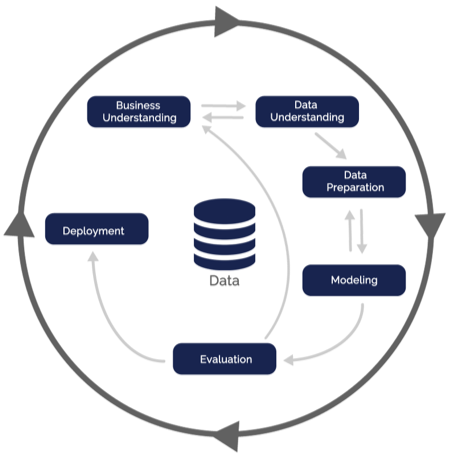
\includegraphics[scale=1.2]{crisp-dm.png}
\caption{Metodología CRISP}
\end{figure}

En el caso de los proyectos de implementación de minería de
datos esta metodología ha representado un grado alto de utilización en desarrollo de estos proyectos.\\

\subsection{Fases}

La metodología incluye un modelo estructurado en seis fases:\\

\begin{enumerate}
\item Compresión del negocio: Es muy importante convertir la información adquirida del negocio en un problema de análisis de datos y que, de igual manera, permita alcanzar los objetivos de negocio propuestos.

Lo que se quiere lograr es asegurar el éxito que tienen algunas de las aplicaciones existentes en Play Store según el sentimiento que les genera a los usuarios a partir de sus críticas.\\


\item Comprensión de los datos:
Las reviews y comentarios que hacen los usuarios en Play Store pueden ser una herramienta de feedback muy poderosa si se interpreta de la manera adecuada y a partir de esa interpretación se toman decisiones que lleven el producto a alcanzar los objetivos esperados.\\


\item Preparación de los datos: 
Para lograr el análisis de éxito de las aplicaciones, se le otorgó importancia al sentimiento que genera cada aplicación para los usuarios (positivo o negativo) y el valor de polaridad y subjetividad de cada crítica.\\


\item Modelado:
La técnica de modelado a utilizar en este caso ha sido elegida en función de los siguientes criterios:\\
Ser adecuada para el problema
Disponer de los datos necesarios para el problema
Cumplir los requisitos del problema
Tiempo necesario para adecuar el modelo\\

Las variables empleadas en la generación del modelo dependen de las características de los datos y la precisión que se quiere lograr con este proyecto.\\


\item Evaluación:
Se evalúa el el modelo teniendo en cuenta los criterios de éxito del problema y conocer si este es útil para las necesidades del negocio.\\


\item Despliegue: Si al evaluar el modelo este comple con las necesidades del negocio y produce los resultados esperados, el modelo ya puede llevarse a cabo para su implementación.

\end{enumerate}

\section{Análisis y Visualización de datos}
Inicialmente, es necesario comprender todos los datos a analizar y el comportamiento de los mismos. Por ende, en la siguiente gráfica logramos representar la forma en que se comporta la polaridad de las reviews respecto a cada sentimiento:\\

\begin{figure}[htb]
\centering
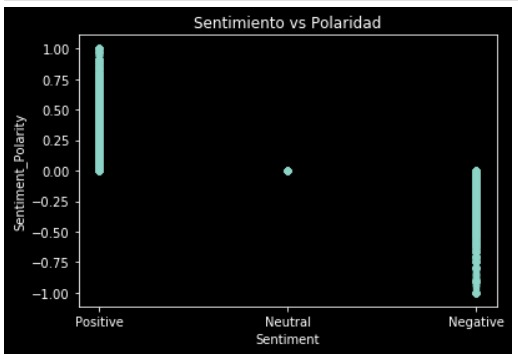
\includegraphics[scale=0.4]{Grafica1.jpg}
\caption{Sentimiento y Polaridad}
\end{figure}
Evidentemente, el valor de la polaridad tiende a representar lógicamente el sentimiento generado en los usuarios. Es decir:
\begin{itemize}
\item Si el valor de polaridad es menor que 0 o negativo el sentimiento es Negativo. 
\item Si el valor de polaridad es igual a 0 el sentimiento es Neutro
\item Si es valor de polaridad es mayor que 0 o positivo el sentimiento es Positivo.\\
\end{itemize}

Para lograr comprender los datos desde la pregunta más lógica: ¿Cuántas reviews positivas y negativas se presentan? Es importante representar los datos a partir de las siguientes gráficas:\\

\begin{figure}[htb]
\centering
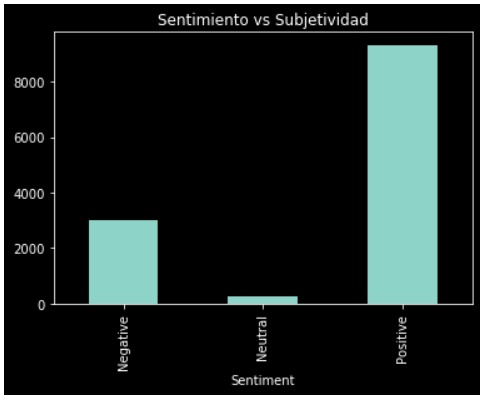
\includegraphics[scale=0.4]{Grafica2.jpg}
\caption{Gráfico de barras Sentimiento y Subjetividad}
\end{figure}
\begin{figure}[htb]
\centering
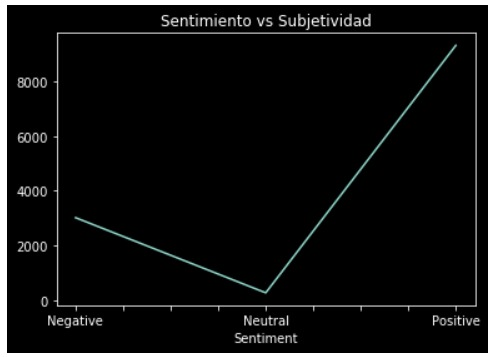
\includegraphics[scale=0.4]{Grafica3.jpg}
\caption{Gráfico líneal Sentimiento y Subjetividad}
\end{figure}

\begin{itemize}
\item Como podemos ver, la cantidad de reviews positivas es mayor que las reviews negativas y/o neutrales.
\item Las review neutrales no serán muy útiles ya que representan menos del 5\% de las reviews totales
\item Las review negativas se deben tener en cuenta, pero, probablemente no aporten demasiado
\end{itemize}

\begin{itemize}
\item La subjetividad del sentimiento de valor positivo debería ser revisado en parte de manera manual.
\item Será necesario equilibrar los datos obtenidos para el modelo.
\item Un tema importante que merece ser tenido en cuenta es la alta concentración de polarización.

\end{itemize}

\section{Conclusiones}
Los datos de las aplicaciones de Play Store tienen un enorme potencial para impulsar al éxito a las empresas de creación de aplicaciones. Se pueden extraer conocimientos prácticos para que los desarrolladores trabajen y capturen el mercado de Android.\\

La metodología de CRISP para proyectos de minería de datos es muy útil para comprender esta tecnología o extraer ideas para diseñar o revisar métodos de trabajo para proyectos con esas características.

\begin{thebibliography}{00}
\bibitem{b1} Galan Cortina, V.(2015). Aplicación de metodología Crisp-DM a un priyecto de minería de datos en el entorno universitario.
\bibitem{b2} [Rodríguez, 2010] Dr. Oldemar Rodríguez Rojas. Metodología para el Desarrollo de Proyectos en Minería de Datos CRISP-DM, 2010.
\bibitem{b3} ESPINOSA-ZUNIGA, Javier Jesús.Aplicación de metodología CRISP-DM para segmentación geográfica de una base de datos pública. Ing. invest. y tecnol. [online]. 2020, vol.21, n.1, e00008.  Epub 03-Ago-2020. ISSN 1405-7743.  https://doi.org/10.22201/fi.25940732e.2020.21n1.008.

\end{thebibliography}

\vspace{12pt}
\color{red} 
URL GitHub:\url{https://github.com/franciscoJavierV/inteligencia_artificial_2021}\\
URL Vídeo:\url{https://youtu.be/C8zc68Gf7Fk}

\end{document}
